\documentclass[11pt, fleqn]{article}

\usepackage{booktabs} % To use /toprule /midrule /bottomrule commands in printing tables
\usepackage{amsmath}
\usepackage{amsfonts}
\usepackage[margin=1in]{geometry} % To set the margin widths
\usepackage{graphicx}
\usepackage{listings}
\usepackage{multirow}
\usepackage{tabularx}
\usepackage{tikz}
\usepackage{varioref}
\usepackage{siunitx}
\usepackage{subcaption}

\lstset{
  language=R,
  literate = {<-}{{$\gets$}}1 {~}{{$\sim$}}1
}
\sisetup{output-exponent-marker=\textsc{e}}

\setlength{\parskip}{12pt} % Sets a blank line in between paragraphs
\setlength\parindent{0pt} % Sets the indent for each paragraph to zero

\begin{document}

\title{Big Data: Homework 2}
\author{Will Clark \& Matthew DeLio \\ 41201-01}
\date{\today}
\maketitle

\section{Data Visualization}

We identified three sets of covariates that affect housing prices:
\begin{enumerate}
\item \textbf{Income/education level:} home price tends to rise with income (and with education, which correlates highly with income);
\item \textbf{Home/neighborhood quality:} nice homes and nice neighborhoods demand a price premium; and
\item \textbf{First-time status:} first-time home buyers tend to purchase less expensive homes.
\end{enumerate}

\subsection{Income \& Education}

Unsurprisingly, buyers with higher income and more education are able to afford more expensive homes. We see in Figure~\vref{fig:hhgrad} that the purchase price of a home increases with each additional level of education achieved. In Figure~\vref{fig:income}, we see that home value rises with income, but much of the variation in income is explained by having a college degree. Red dots, signifying purchasers with a college or graduate degree, are concentrated in the northeast corner, signifying high incomes and expensive homes. Blue dots, signifying purchasers without a college degree, have lower incomes and (expectedly) less expensive homes.

\begin{figure}
  \centering
  \begin{subfigure}[b]{0.49\textwidth}
    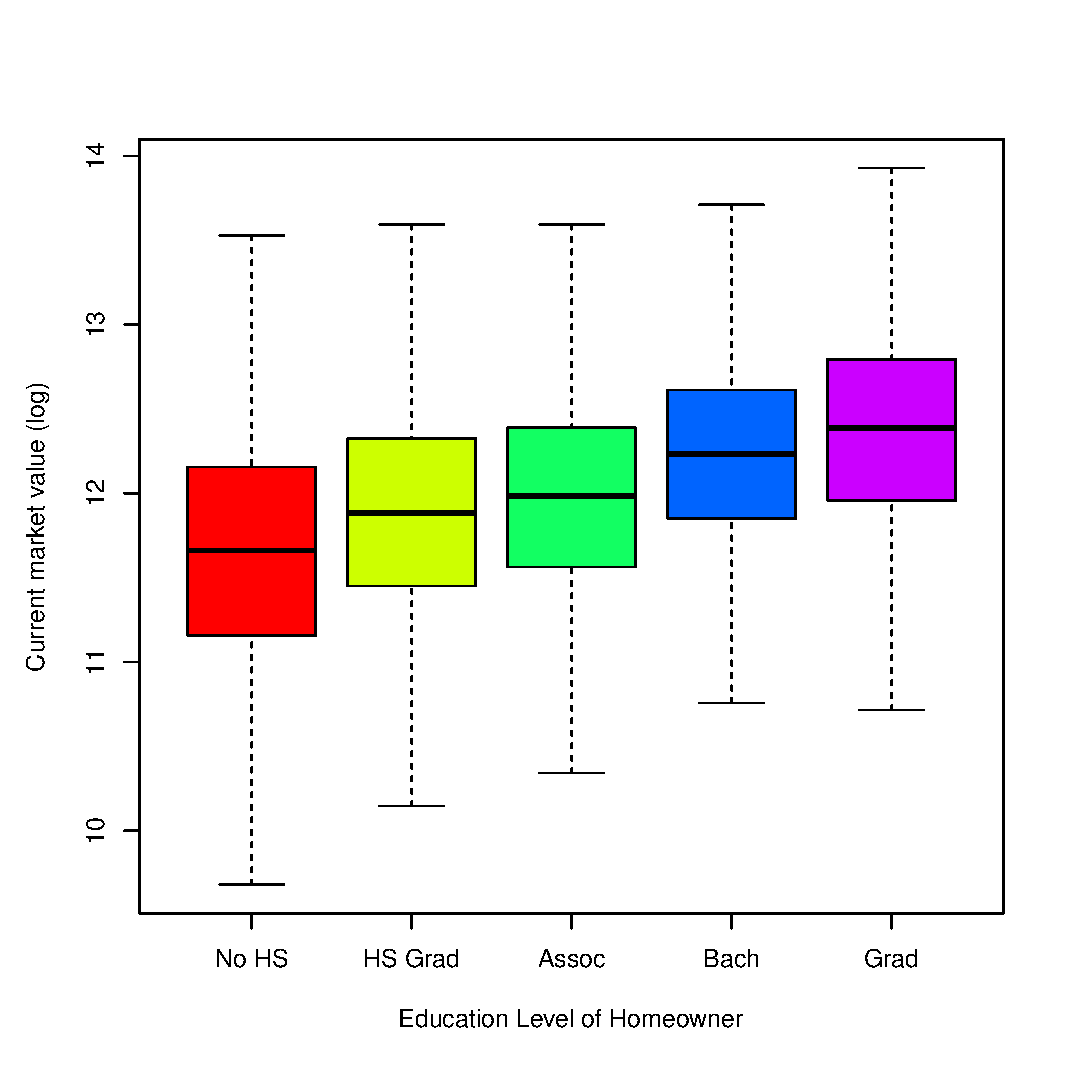
\includegraphics[width=\textwidth]{hhgrad.eps}
    \caption{Home Value and Education}
    \label{fig:hhgrad}
  \end{subfigure}
  \hfill
  \begin{subfigure}[b]{0.49\textwidth}
    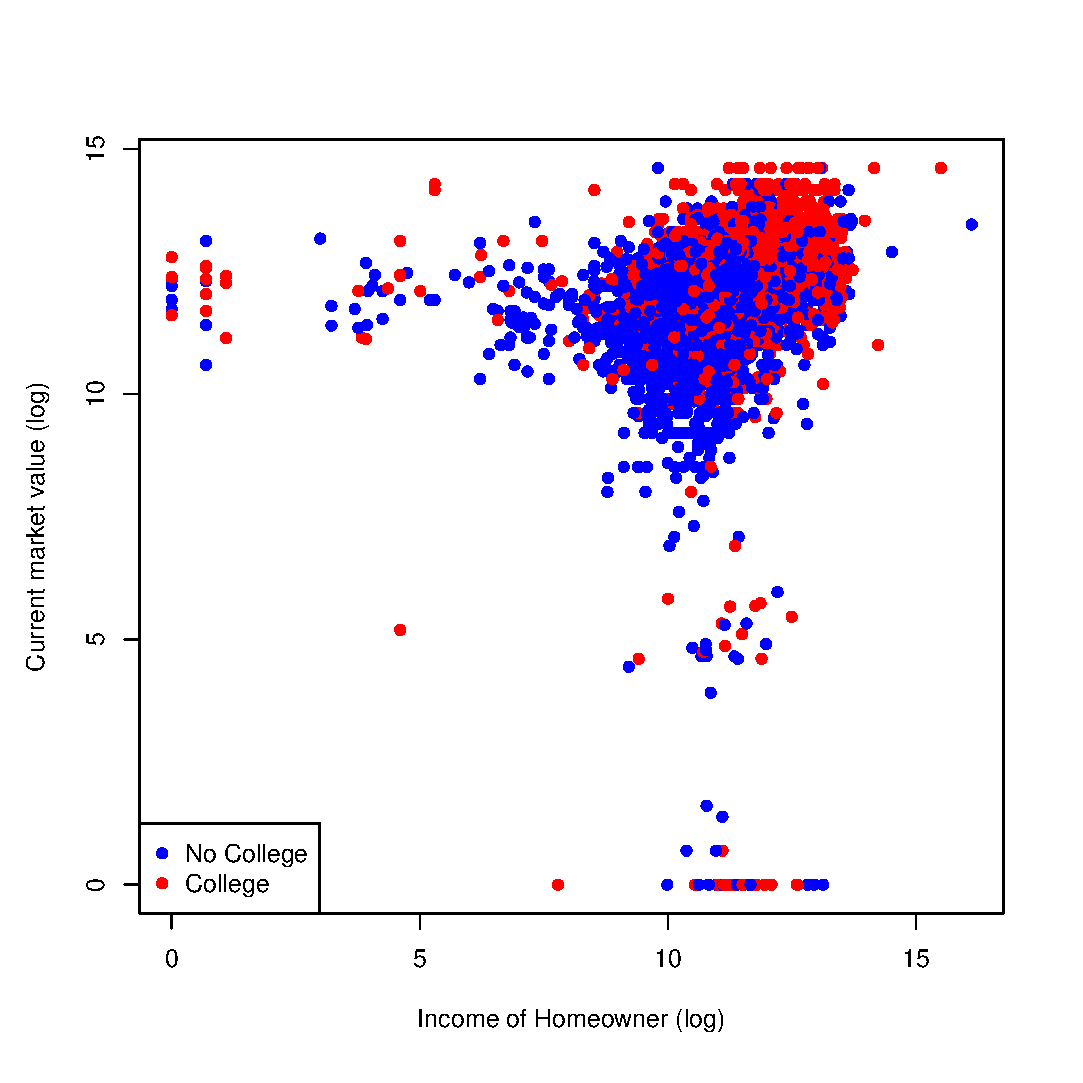
\includegraphics[width=\textwidth]{income.eps}
    \caption{Home Value and Income}
    \label{fig:income}
  \end{subfigure}
  \caption{Education and Income}
\end{figure}

In addition to more expensive homes, more education correlates with neighborhood quality. Figure~\vref{fig:education_qual} shows the share of households by terminal degree level in good and bad neighborhoods. More educated buyers are more likely to have homes in good neighborhoods; we expect that this is really an income story, as education increases income which affords higher neighborhood quality.

\begin{figure}[!htb]
  \centering
  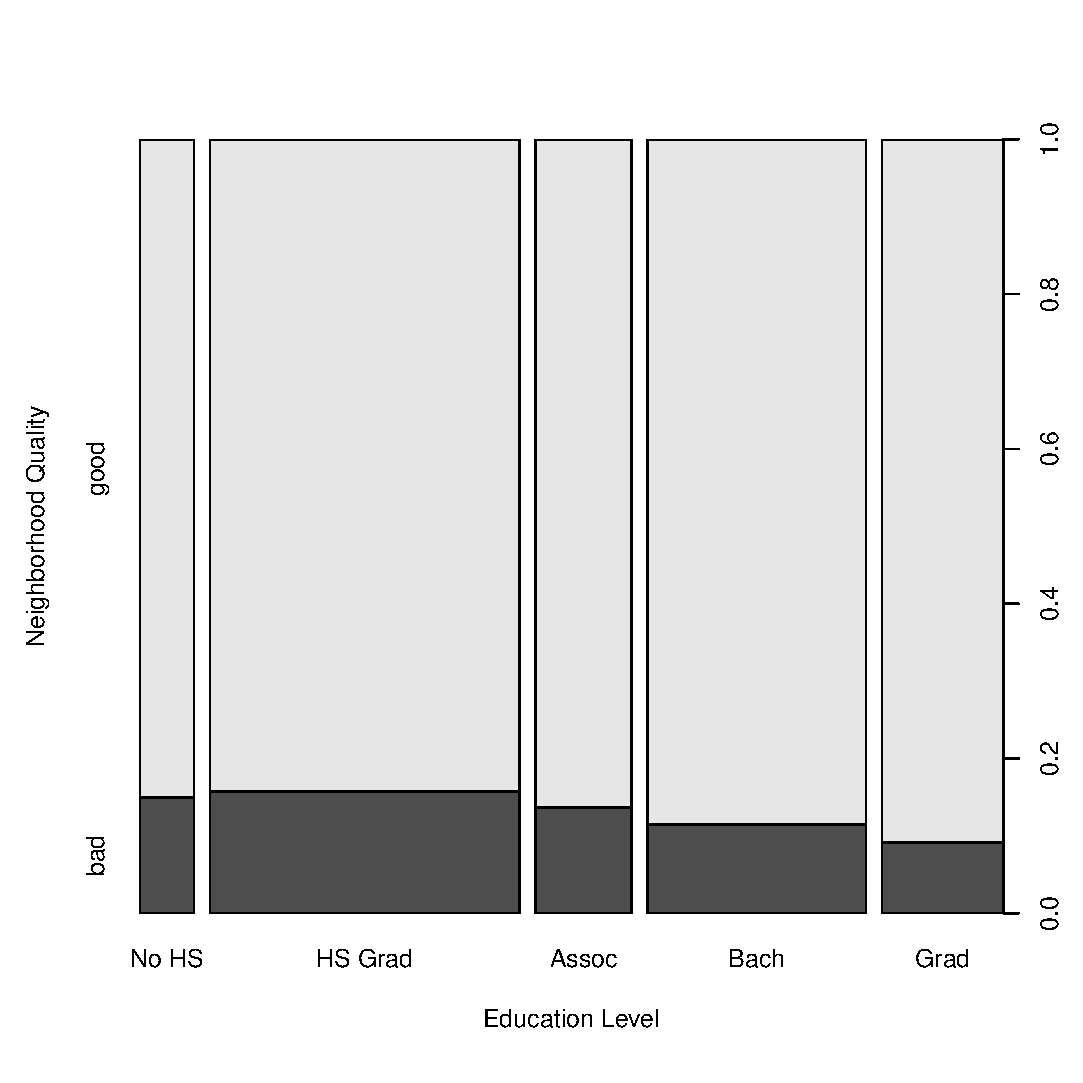
\includegraphics[scale=.5]{neighborhood_quality_vs_education.eps}
  \caption{Neighborhood Quality and Income}
  \label{fig:education_qual}
\end{figure}

\subsection{Neighborhood \& Home}

The value of a home is also driven by the quality of the home and the surrounding neighborhood. We expect that nicer homes in nicer neighborhoods will cost more. We see in Figure~\vref{fig:ejunk} and Figure~\vref{fig:eaban} that two proxies for neighborhood quality\textemdash the presence of junk in the street and proximity to abandoned buildings\textemdash both lower home value. 

\begin{figure}
  \centering
  \begin{subfigure}[b]{0.49\textwidth}
    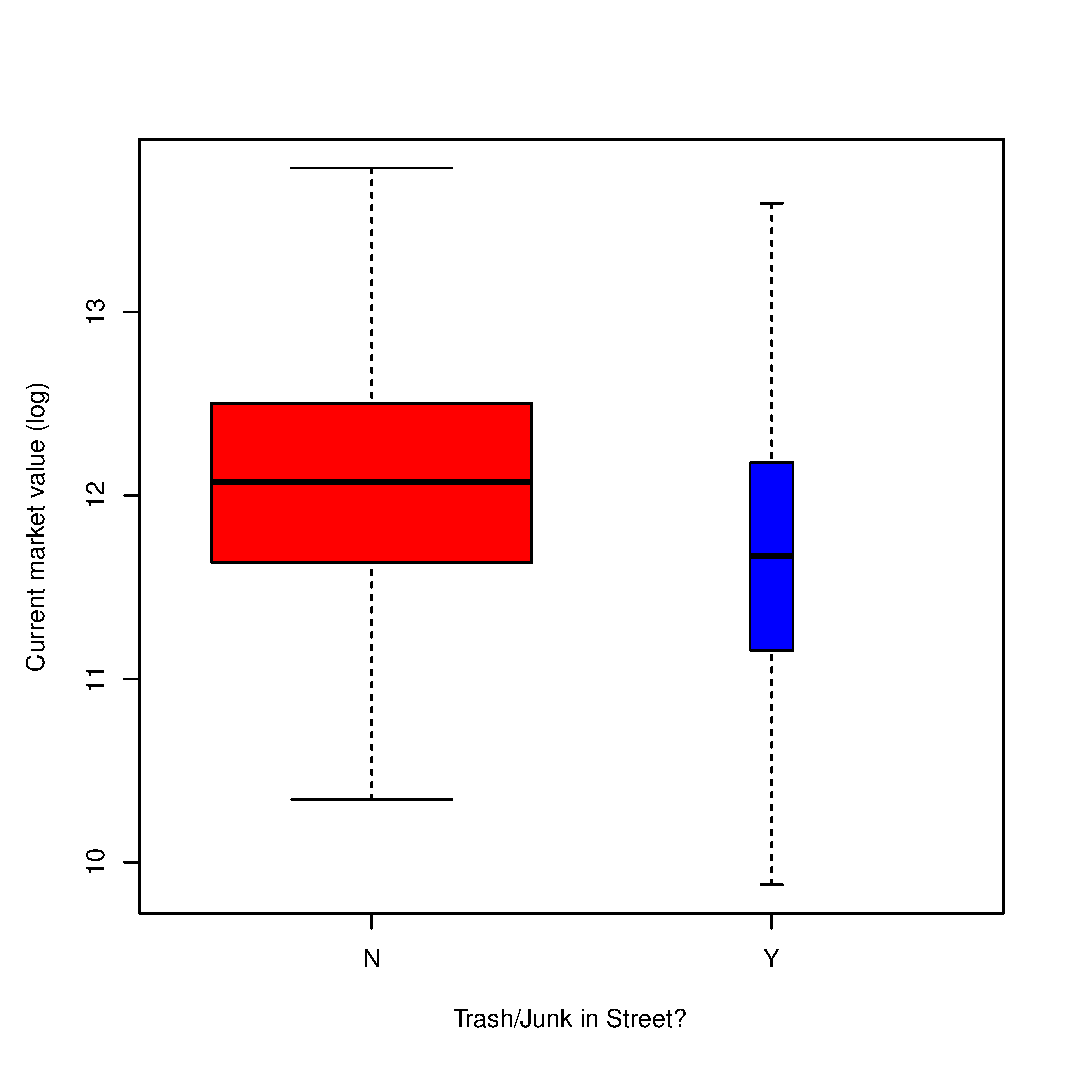
\includegraphics[width=\textwidth]{ejunk.eps}
    \caption{Near Street Trash}
    \label{fig:ejunk}
  \end{subfigure}
  \hfill
  \begin{subfigure}[b]{0.49\textwidth}
    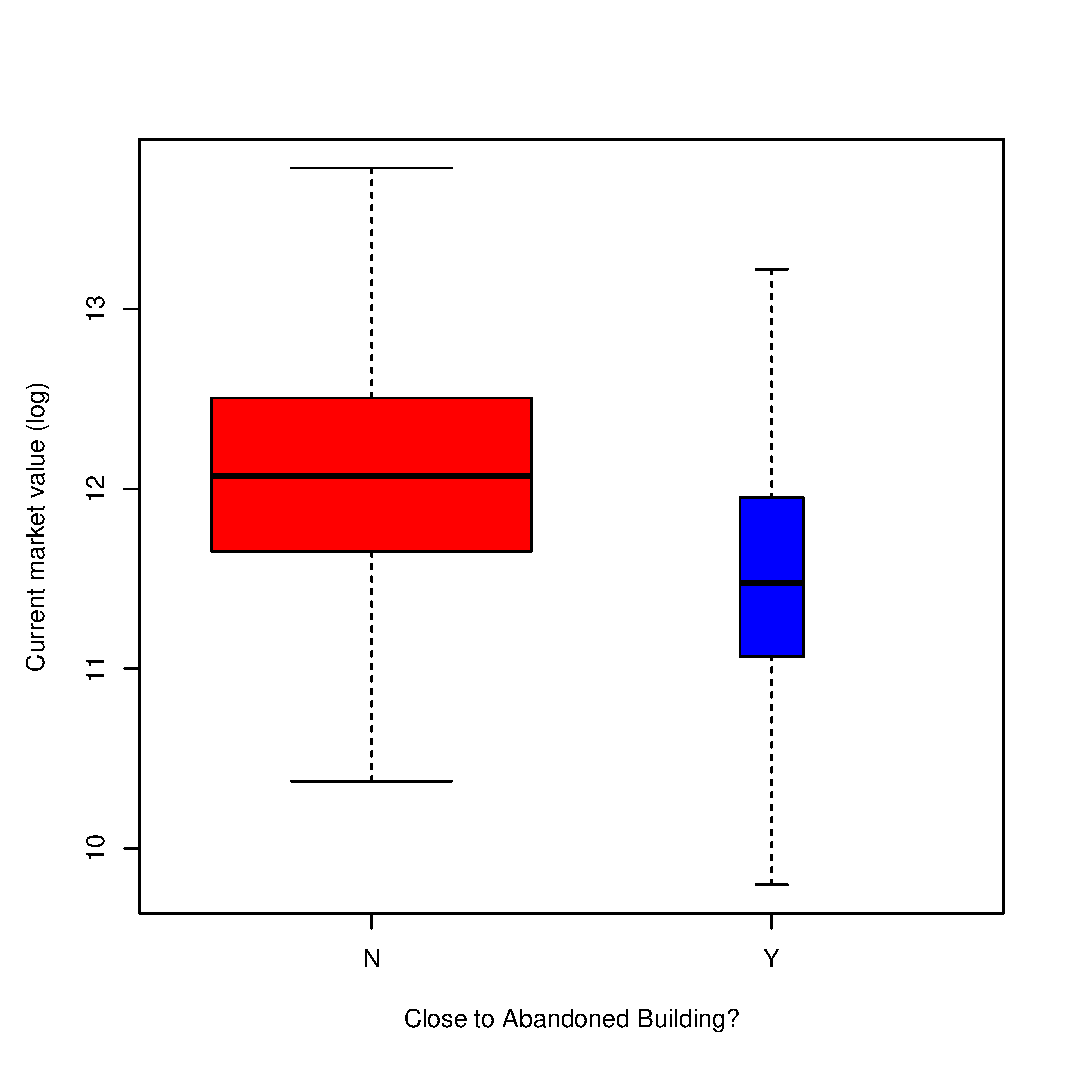
\includegraphics[width=\textwidth]{eaban.eps}
    \caption{Near Abandoned Buildings}
    \label{fig:eaban}
  \end{subfigure}
  \caption{Neighborhood Quality}
\end{figure}

As we would expect, homes that are identified as ``good'' quality cost more than those that are not, and good neighborhoods carry a premium over bad neighborhoods (Figure~\ref{fig:howh} and Figure~\ref{fig:hown}, respectively).

\begin{figure}
  \centering
  \begin{subfigure}[b]{0.49\textwidth}
    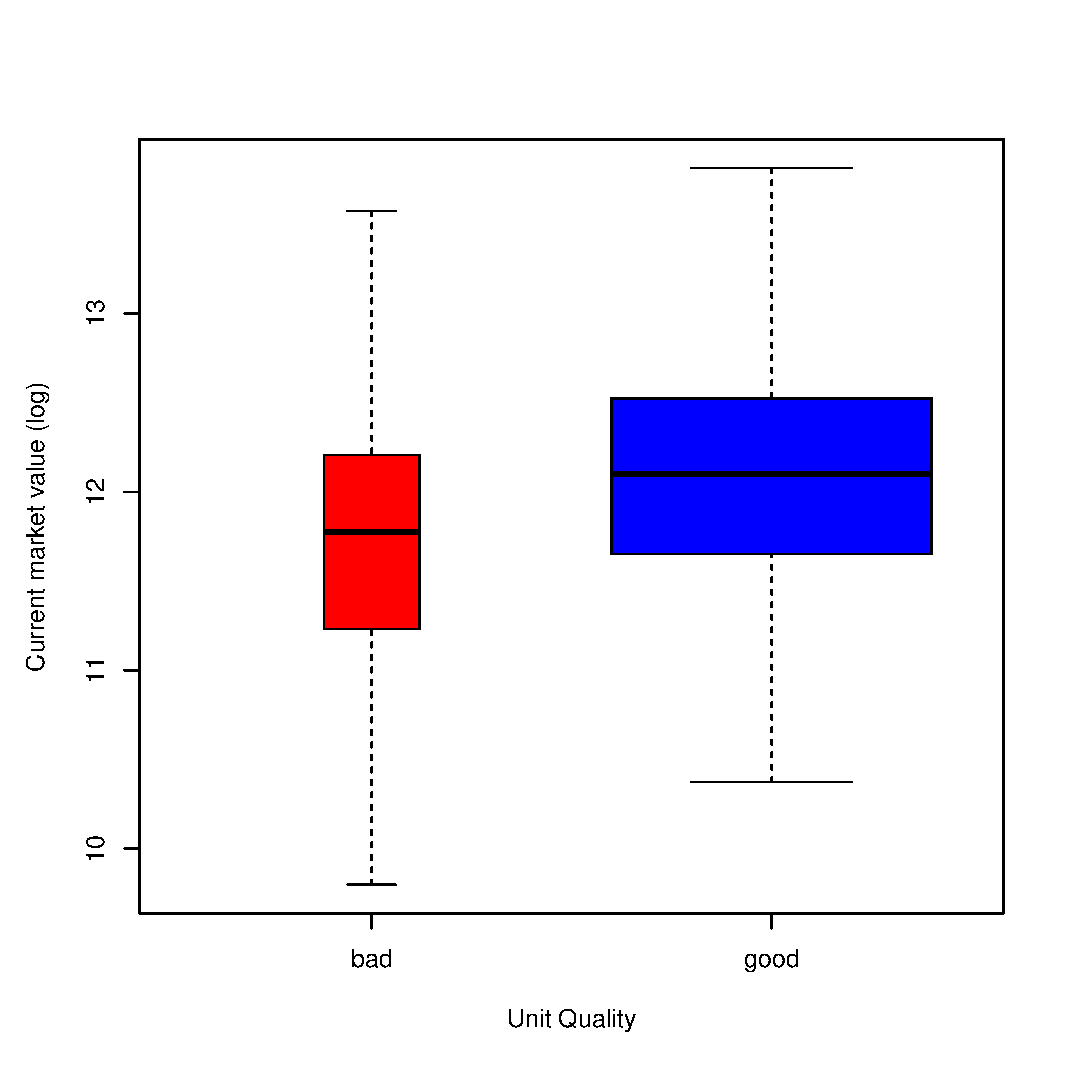
\includegraphics[width=\textwidth]{howh.eps}
    \caption{Home Ratings}
    \label{fig:howh}
  \end{subfigure}
  \hfill
  \begin{subfigure}[b]{0.49\textwidth}
    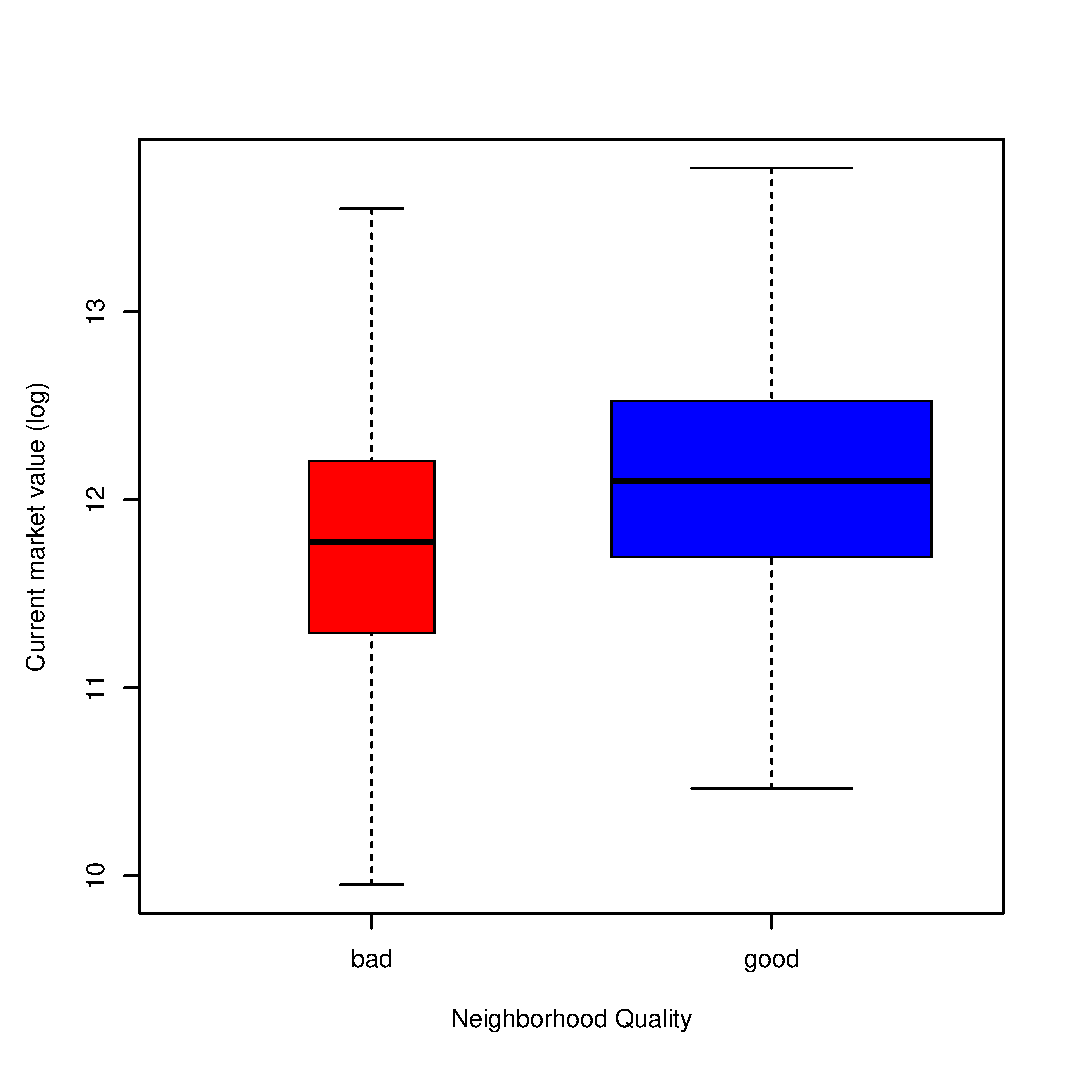
\includegraphics[width=\textwidth]{hown.eps}
    \caption{Neighborhood Ratings}
    \label{fig:hown}
  \end{subfigure}
  \caption{Home and Neighborhood Quality}
\end{figure}

We can begin looking at the difference between first-time and repeat home buyers through this lens as well. We see in Figure~\vref{fig:first_qual} that first-time home buyers are more likely than not to purchase a home with a ``bad'' rating, while repeat purchasers are more likely to purchase a home with a ``good''rating. In the next section, we look more closely at the characteristics of first-time buyers that could explain this quality difference.

\begin{figure}[!htb]
  \centering
  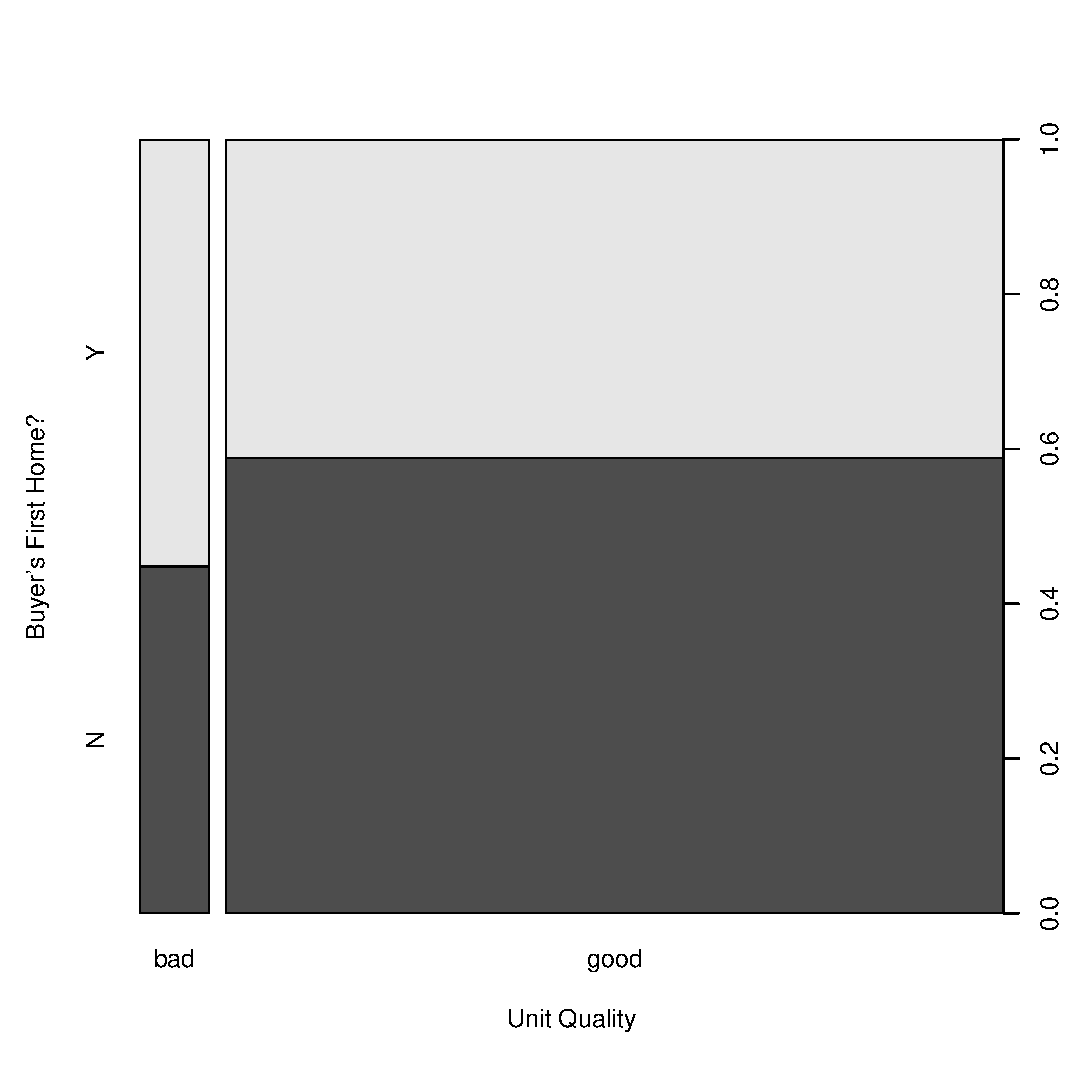
\includegraphics[scale=.5]{first_home_vs_home_quality.eps}
  \caption{Unit Quality for First-Time Buyers}
  \label{fig:first_qual}
\end{figure}

\subsection{First-time Buyers \& Financing Source}

Finally, we examine the difference paid for first-time home buyers versus repeat home buyers. We have two different data sources that tell a similar story. First, buyers who are purchasing their first home tend to pay less than those who are buying a second (or third) home (see Figure~\vref{fig:frstho}). We expect that this is due to age and income differences; first-time home buyers will tend to be younger and have less accumulated wealth than repeat buyers. 

We see that the source of financing for a down payment tells a very similar story. Buyers that use a previous home to pay down their purchase buy more expensive homes (see Figure~\vref{fig:dwnpay}). We expect that this is capturing the same effect as described above: namely, that if a previous home is used as a source of financing, that signals an older buyer with higher income and greater wealth.

\begin{figure}
  \centering
  \begin{subfigure}[b]{0.49\textwidth}
    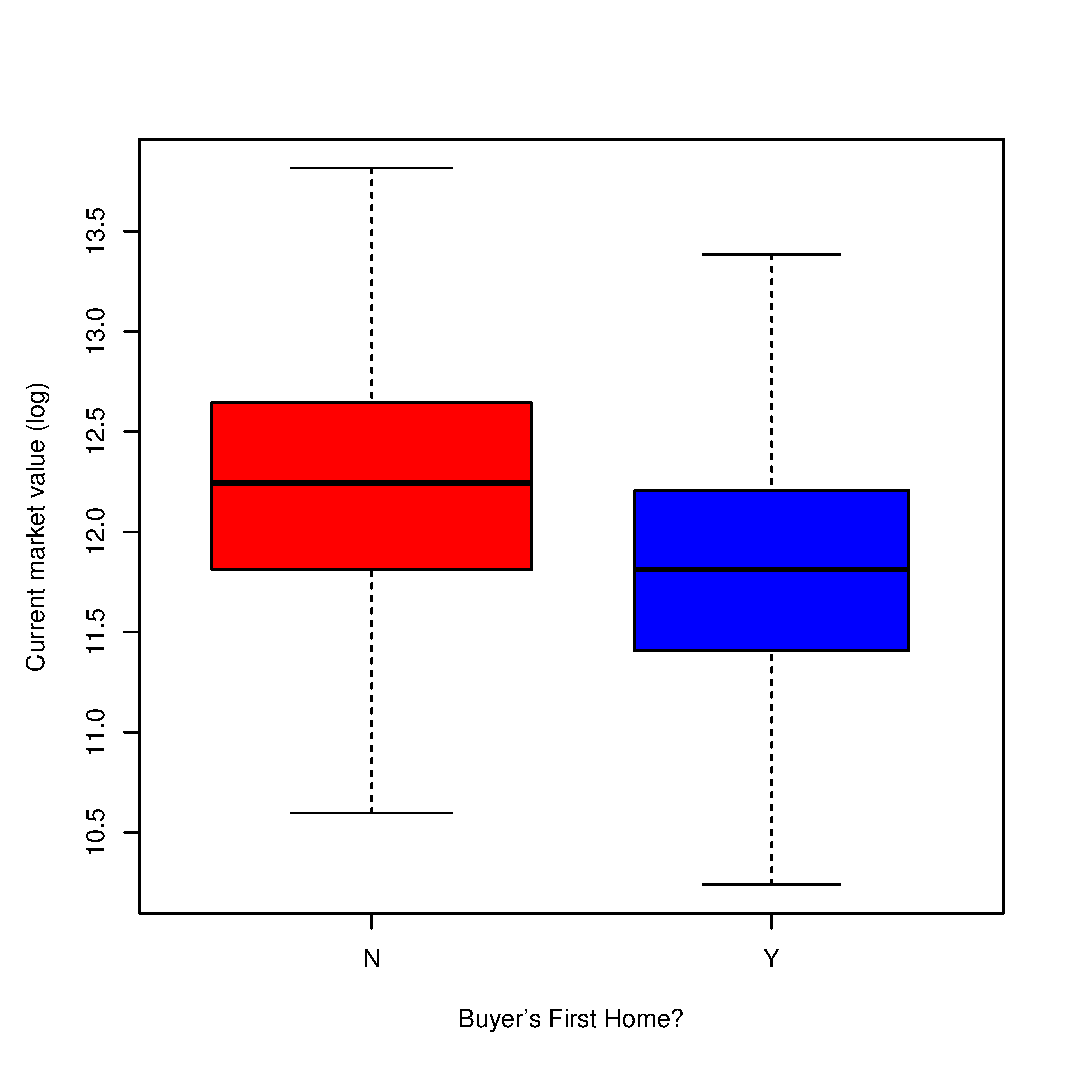
\includegraphics[width=\textwidth]{frstho.eps}
    \caption{First-Time Buyers}
    \label{fig:frstho}
  \end{subfigure}
  \hfill
  \begin{subfigure}[b]{0.49\textwidth}
    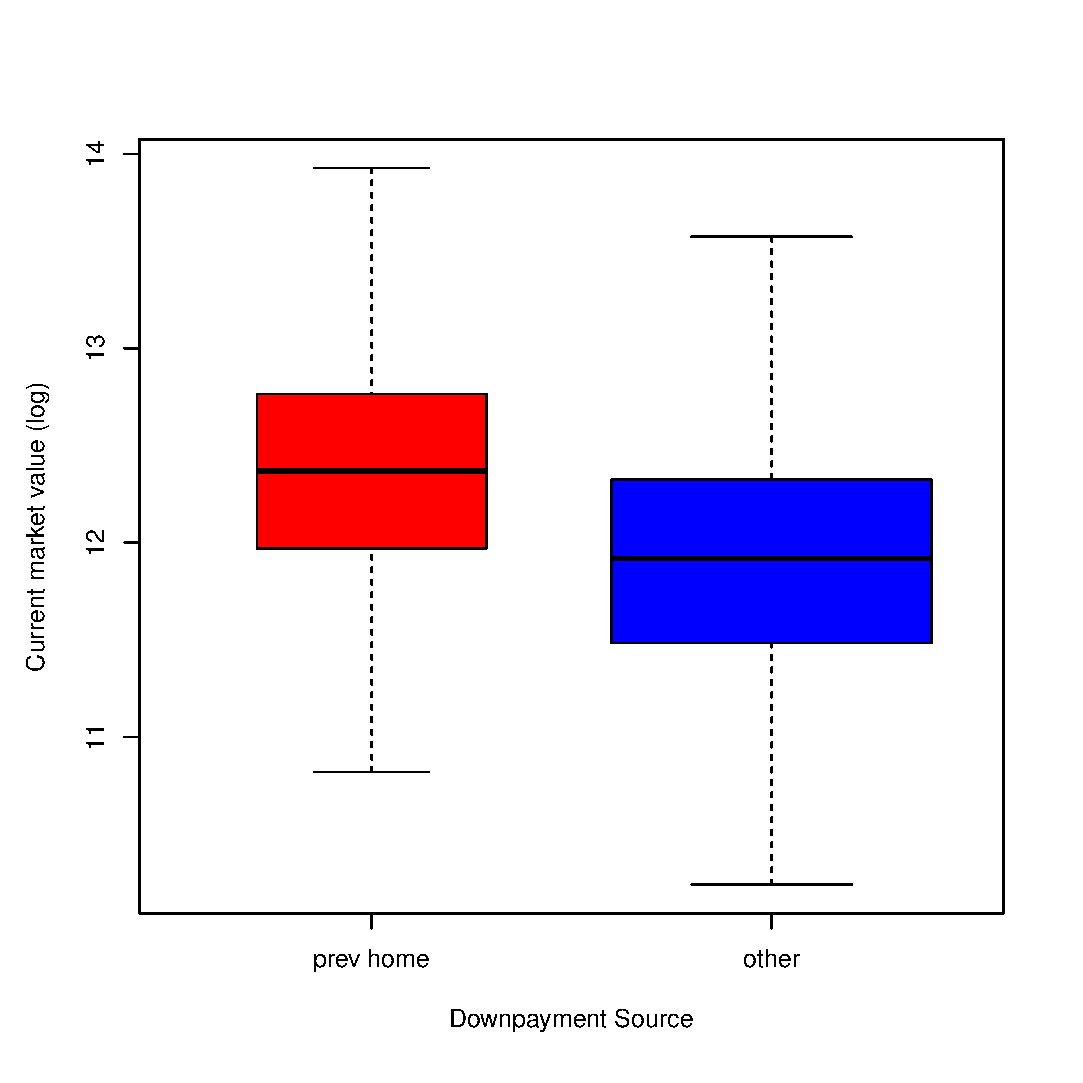
\includegraphics[width=\textwidth]{dwnpay.eps}
    \caption{Mortgage Financing}
    \label{fig:dwnpay}
  \end{subfigure}
  \caption{Repeat Purchaser Status and Financing}
\end{figure}

\section{Linear Model}

We begin by regressing the log of home value onto all possible co-variates (excluding mortgage amount and purchase price, which are known functions of home value). If we apply a false discovery rate of 10 percent, we find that there are 34 true discoveries. We regress log of home value on these 34 covariates; the results are displayed in Table~\vref{tab:reg1_fdr}.

The model fit does not change meaningfully between estimates; the R-squared of the first model is 0.3053 and the R-squared of the second model is 0.3050. Removing the extraneous covariates should give us more accurate estimates for the effects of each covariate on home value.

Some notes on the linear regression model:
\begin{itemize}
  \item Every state included in the model (there were 13) is a significant covariate. California is the most expensive state; Texas is the cheapest.
  \item More education increases the value of home purchased, but income seems to have very little effect (that is not already included in education).
  \item Number of bedrooms and bathrooms both increase home value, but the relationship is stronger for number of bathrooms (i.e. it is the best proxy of home size).
  \item The neighborhood and home quality measures that we saw in the first section appear in our regression results. Junk in the street lowers home value, as do nearby abandoned buildings. Good homes and neighborhoods cost more than bad ones.
\end{itemize}

% latex table generated in R 3.1.2 by xtable 1.7-4 package
% Thu Apr 16 19:27:00 2015
\begin{table}[ht]
\centering
\begin{tabular}{rrrrr}
  \hline
 & Estimate & Std. Error & t value & Pr($>$$|$t$|$) \\ 
  \hline
(Intercept) & 11.5901 & 0.0606 & 191.21 & 0.0000 \\ 
  EAPTBLY & -0.0446 & 0.0221 & -2.02 & 0.0436 \\ 
  ECOM2Y & -0.0985 & 0.0470 & -2.10 & 0.0361 \\ 
  EJUNKY & -0.1258 & 0.0509 & -2.47 & 0.0134 \\ 
  ESFDY & 0.2884 & 0.0292 & 9.86 & 0.0000 \\ 
  EABANY & -0.1633 & 0.0359 & -4.55 & 0.0000 \\ 
  HOWHgood & 0.1292 & 0.0263 & 4.92 & 0.0000 \\ 
  HOWNgood & 0.1197 & 0.0219 & 5.47 & 0.0000 \\ 
  STRNAY & -0.0391 & 0.0158 & -2.47 & 0.0136 \\ 
  ZINC2 & 0.0000 & 0.0000 & 11.24 & 0.0000 \\ 
  HHGRADBach & 0.1333 & 0.0229 & 5.82 & 0.0000 \\ 
  HHGRADGrad & 0.1979 & 0.0257 & 7.69 & 0.0000 \\ 
  `HHGRADHS Grad` & -0.0615 & 0.0217 & -2.84 & 0.0046 \\ 
  `HHGRADNo HS` & -0.1971 & 0.0318 & -6.20 & 0.0000 \\ 
  NUNITS & -0.0010 & 0.0005 & -1.87 & 0.0610 \\ 
  INTW & -0.0469 & 0.0044 & -10.66 & 0.0000 \\ 
  METROurban & 0.0837 & 0.0179 & 4.67 & 0.0000 \\ 
  STATECO & -0.2876 & 0.0290 & -9.91 & 0.0000 \\ 
  STATECT & -0.3444 & 0.0312 & -11.04 & 0.0000 \\ 
  STATEGA & -0.6555 & 0.0309 & -21.20 & 0.0000 \\ 
  STATEIL & -0.8624 & 0.0576 & -14.96 & 0.0000 \\ 
  STATEIN & -0.7779 & 0.0307 & -25.37 & 0.0000 \\ 
  STATELA & -0.7218 & 0.0368 & -19.63 & 0.0000 \\ 
  STATEMO & -0.6647 & 0.0334 & -19.89 & 0.0000 \\ 
  STATEOH & -0.6762 & 0.0326 & -20.73 & 0.0000 \\ 
  STATEOK & -0.9978 & 0.0328 & -30.43 & 0.0000 \\ 
  STATEPA & -0.8681 & 0.0338 & -25.67 & 0.0000 \\ 
  STATETX & -1.0497 & 0.0343 & -30.64 & 0.0000 \\ 
  STATEWA & -0.1203 & 0.0309 & -3.89 & 0.0001 \\ 
  BATHS & 0.2134 & 0.0116 & 18.46 & 0.0000 \\ 
  BEDRMS & 0.0877 & 0.0094 & 9.35 & 0.0000 \\ 
  MATBUYY & -0.0277 & 0.0136 & -2.03 & 0.0421 \\ 
  `DWNPAYprev home` & 0.1215 & 0.0178 & 6.81 & 0.0000 \\ 
  FRSTHOY & -0.0829 & 0.0172 & -4.82 & 0.0000 \\ 
   \hline
\end{tabular}
\caption{Value of Purchased Homes (in logs)} 
\label{tab:reg1_fdr}
\end{table}


\section{Logistic Model}
For this model, we regress, using the same covariates as the linear model, whether or not a home-buyer had a down payment of 20\% or more when purchasing a home.  As before we apply a false discovery rate of 10\%, and find that there are 23 true discoveries.  We again, applied the same regression using these 23 covariates with the results shown in Table~\vref{tab:reg3_fdr}.

% latex table generated in R 3.1.2 by xtable 1.7-4 package
% Fri Apr 17 00:56:45 2015
\begin{table}[ht]
\centering
\begin{tabular}{rrrrr}
  \hline
 & Estimate & Std. Error & t value & Pr($>$$|$t$|$) \\ 
  \hline
(Intercept) & 0.1925 & 0.0261 & 7.37 & 0.0000 \\ 
  ECOM1Y & -0.0285 & 0.0096 & -2.96 & 0.0031 \\ 
  ECOM2Y & -0.0439 & 0.0248 & -1.77 & 0.0763 \\ 
  ESFDY & -0.0566 & 0.0151 & -3.74 & 0.0002 \\ 
  HOWNgood & 0.0166 & 0.0105 & 1.59 & 0.1122 \\ 
  STRNAY & -0.0164 & 0.0083 & -1.97 & 0.0489 \\ 
  PER & -0.0208 & 0.0025 & -8.34 & 0.0000 \\ 
  HHGRADBach & 0.0354 & 0.0082 & 4.31 & 0.0000 \\ 
  HHGRADGrad & 0.0563 & 0.0103 & 5.45 & 0.0000 \\ 
  INTW & -0.0094 & 0.0023 & -4.11 & 0.0000 \\ 
  STATECT & 0.1423 & 0.0128 & 11.08 & 0.0000 \\ 
  STATEGA & -0.0476 & 0.0130 & -3.66 & 0.0003 \\ 
  STATEIL & 0.1045 & 0.0286 & 3.66 & 0.0003 \\ 
  STATEIN & 0.0332 & 0.0127 & 2.61 & 0.0091 \\ 
  STATELA & 0.0953 & 0.0166 & 5.73 & 0.0000 \\ 
  STATEMO & 0.0926 & 0.0146 & 6.36 & 0.0000 \\ 
  STATEOH & 0.1342 & 0.0139 & 9.63 & 0.0000 \\ 
  STATEPA & 0.1028 & 0.0148 & 6.96 & 0.0000 \\ 
  STATETX & 0.0406 & 0.0148 & 2.75 & 0.0059 \\ 
  BATHS & 0.0433 & 0.0058 & 7.49 & 0.0000 \\ 
  MATBUYY & 0.0493 & 0.0071 & 6.94 & 0.0000 \\ 
  `DWNPAYprev home` & 0.1605 & 0.0094 & 17.15 & 0.0000 \\ 
  VALUE & 0.0000 & 0.0000 & 12.89 & 0.0000 \\ 
  FRSTHOY & -0.0579 & 0.0090 & -6.43 & 0.0000 \\ 
   \hline
\end{tabular}
\caption{Probability of Down Payment $>$ 20\% (No Interaction Terms)} 
\label{tab:reg3_fdr}
\end{table}


\subsection{Interpret Effects}
The effects of two of the variables, one a factor (``FRSTHOY'') the other continuous (``BATHS'') yields some insights into the logistic regression model as a whole.  The following is a simplification of the model that will be used to discuss the interpretation of these variables:

\math{
  logit(p) = log(\frac{p}{1-p}) = \beta_0 + ... + \beta_{FRSTHOY}FRSTHOY + \beta_{BATHS}BATHS
}

Holding all other covariates fixed (including ``BATHS''), we first examine the effects of being a first-time home-buyer (``FRSTHOY==TRUE'').  From the definition of the logit we know that being a first-time home-buyer will have the following effect: $odds(p)=p/(1-p)=\exp(\beta_{FRSTHOY})=\exp(-0.0579)=0.943$.  In other words, being a first-time home-buyer will decrease the odds by $\sim5.6\%$ that a $>20\%$ down-payment was made.  This is unsurprising since as we mentioned earlier, first-time home-buyers tend to have less wealth than people who have owned homes in the past.

Turning our attention now to the number of baths in a house, we can perform a similar analysis.  Again from the logit definition $odds(p)=\exp(0.0433)=1.044$.  Put another way, each additional bath will increase the odds of having a $>20\%$ down-payment by $\sim4.4\%$.

\subsection{Interpret Interaction}
A new model was formed to include determine the interaction between the buyer's first home and the number of baths in predicting the down-payment.

\begin{lstlisting}[language=R]
model <- glm(gt20dwn ~ . - AMMORT - LPRICE + FRSTHO*BATHS, 
             data=homes, family='binomial')
\end{lstlisting}

As before we apply a false discovery rate of 10\%, and find 23 covariates above the threshold.  We then created a final model using these covariates; the results are shown in Table~\vref{tab:reg4_fdr}.  It is worth noting in that table, that FRSTHOY's effect on the intercept has been eliminated during the false discovery rate detection and is not included in the model.  However, the interaction term ``BATHS:FRSTHOY'' is included.  The following is a simplification of the model that will be used to discuss the interpretation of the interaction variables:

\math{
  logit(p) = \beta_0 + ... + (\beta_{BATHS} + \beta_{BATHS:FRSTHOY}FRSTHOY) * BATHS
}

Interpreting these coefficients and their effects on the log-odds is similar to the situation discussed earlier.  If not a first-time buyer, each bath will have the following effect on the odds:  $odds(p)=\exp(\beta_{BATHS})=\exp(0.0556) = 1.057$, or a $\sim5.7\%$ increase in the odds that $>20\%$ was made.  However, if a first-time home-buyer purchases a house, each additional bath will have the following effect: $odds(p)=\exp(\beta_{BATHS}+\beta_{BATHS:FRSTHOY})=\exp(0.0556-0.0367)=1.019$, or a $\sim1.9\%$ increase in odds.  Put another way, with respect to the number of baths (as a proxy for the value of the house), first-time home-buyers are less likely to have a substantial down-payment when houses have more value.  Again, this agrees with our notion that first-time home-buyers have less wealth to put into a home purchase.

% latex table generated in R 3.1.2 by xtable 1.7-4 package
% Thu Apr 16 19:10:20 2015
\begin{table}[ht]
\centering
\begin{tabular}{rrrrr}
  \hline
 & Estimate & Std. Error & t value & Pr($>$$|$t$|$) \\ 
  \hline
(Intercept) & 0.1766 & 0.0255 & 6.92 & 0.0000 \\ 
  ECOM1Y & -0.0284 & 0.0096 & -2.94 & 0.0032 \\ 
  ECOM2Y & -0.0449 & 0.0248 & -1.81 & 0.0700 \\ 
  ESFDY & -0.0573 & 0.0151 & -3.79 & 0.0002 \\ 
  HOWNgood & 0.0174 & 0.0105 & 1.67 & 0.0957 \\ 
  STRNAY & -0.0166 & 0.0083 & -1.99 & 0.0462 \\ 
  PER & -0.0208 & 0.0025 & -8.35 & 0.0000 \\ 
  HHGRADBach & 0.0358 & 0.0082 & 4.36 & 0.0000 \\ 
  HHGRADGrad & 0.0566 & 0.0103 & 5.48 & 0.0000 \\ 
  INTW & -0.0097 & 0.0023 & -4.22 & 0.0000 \\ 
  STATECT & 0.1411 & 0.0128 & 11.00 & 0.0000 \\ 
  STATEGA & -0.0473 & 0.0130 & -3.64 & 0.0003 \\ 
  STATEIL & 0.1024 & 0.0286 & 3.59 & 0.0003 \\ 
  STATEIN & 0.0324 & 0.0127 & 2.55 & 0.0109 \\ 
  STATELA & 0.0955 & 0.0166 & 5.74 & 0.0000 \\ 
  STATEMO & 0.0910 & 0.0145 & 6.25 & 0.0000 \\ 
  STATEOH & 0.1324 & 0.0139 & 9.50 & 0.0000 \\ 
  STATEPA & 0.0999 & 0.0148 & 6.77 & 0.0000 \\ 
  STATETX & 0.0397 & 0.0147 & 2.69 & 0.0071 \\ 
  BATHS & 0.0556 & 0.0058 & 9.52 & 0.0000 \\ 
  MATBUYY & 0.0493 & 0.0071 & 6.95 & 0.0000 \\ 
  `DWNPAYprev home` & 0.1553 & 0.0092 & 16.84 & 0.0000 \\ 
  VALUE & 0.0000 & 0.0000 & 12.35 & 0.0000 \\ 
  `BATHS:FRSTHOY` & -0.0367 & 0.0047 & -7.75 & 0.0000 \\ 
   \hline
\end{tabular}
\caption{Probability of Down Payment $>$ 20\% (With Interaction Term)} 
\label{tab:reg4_fdr}
\end{table}


\section{Out-of-Sample Prediction}
\subsection{Predicting Down-Payments on Homes $<100k$}
Here we create a new model that is trained using data for home values $>100k$, which will then be used to predict the $20\%$ down-payment rate for homes worth $<100k$.  We begin by including using all covariates and including the interaction between first-time home-buyers and # of baths from the previous section.  Again, using a 10\% false discovery rate cutoff, 23 covariates are significant and included in the final model (see Table~\vref{tab:reg6_fdr}).  From the coefficients, we clearly see more pronounced effects for the number of baths and first-time home-buyers.  For a first-time home-buyer of a home whose value is $>100k$ each bath will increase the odds of having a substantial down-payment by $\sim9.7\%$.  For a seasoned home-buyer these odds increase to $\sim31.3\%$.

% latex table generated in R 3.1.2 by xtable 1.7-4 package
% Fri Apr 17 02:05:13 2015
\begin{table}[ht]
\centering
\begin{tabular}{rrrrr}
  \hline
 & Estimate & Std. Error & z value & Pr($>$$|$z$|$) \\ 
  \hline
(Intercept) & -1.5396 & 0.1686 & -9.13 & 0.0000 \\ 
  ECOM1Y & -0.1052 & 0.0637 & -1.65 & 0.0989 \\ 
  ECOM2Y & -0.4255 & 0.2045 & -2.08 & 0.0375 \\ 
  ESFDY & -0.3880 & 0.0952 & -4.07 & 0.0000 \\ 
  HOWNgood & 0.1830 & 0.0749 & 2.44 & 0.0146 \\ 
  STRNAY & -0.1203 & 0.0536 & -2.24 & 0.0249 \\ 
  PER & -0.1262 & 0.0159 & -7.92 & 0.0000 \\ 
  HHGRADBach & 0.2060 & 0.0481 & 4.29 & 0.0000 \\ 
  HHGRADGrad & 0.2840 & 0.0576 & 4.93 & 0.0000 \\ 
  INTW & -0.0629 & 0.0170 & -3.70 & 0.0002 \\ 
  STATECT & 0.7022 & 0.0713 & 9.85 & 0.0000 \\ 
  STATEGA & -0.3185 & 0.0790 & -4.03 & 0.0001 \\ 
  STATEIL & 0.4888 & 0.1873 & 2.61 & 0.0091 \\ 
  STATEIN & 0.2181 & 0.0804 & 2.71 & 0.0067 \\ 
  STATELA & 0.5780 & 0.1052 & 5.49 & 0.0000 \\ 
  STATEMO & 0.5182 & 0.0865 & 5.99 & 0.0000 \\ 
  STATEOH & 0.6956 & 0.0824 & 8.45 & 0.0000 \\ 
  STATEPA & 0.6664 & 0.0996 & 6.69 & 0.0000 \\ 
  STATETX & 0.2843 & 0.1095 & 2.60 & 0.0094 \\ 
  BATHS & 0.2722 & 0.0342 & 7.96 & 0.0000 \\ 
  MATBUYY & 0.3485 & 0.0430 & 8.11 & 0.0000 \\ 
  `DWNPAYprev home` & 0.7872 & 0.0519 & 15.17 & 0.0000 \\ 
  VALUE & 0.0000 & 0.0000 & 11.09 & 0.0000 \\ 
  `BATHS:FRSTHOY` & -0.1797 & 0.0297 & -6.05 & 0.0000 \\ 
   \hline
\end{tabular}
\caption{Probability of Down Payment $>20\%$ (for Home Value $>100k$)} 
\label{tab:reg6_fdr}
\end{table}


We then use this model to predict some out-of-sample homes with value $<100k$.  These results are shown in Figure~\vref{fig:oos_lt100k}.  Looking that this figure more carefully we see that our model correctly predicts most of the times when the actual down payment is $<20\%$ (both our 3rd quartile and statistical max are well below the 0.5 threshold).  However, when the down-payment is $>20\%$ we mis-predict it to be false; our statistical min and 1st/3rd quartiles are well below 0.5 and the max is just above at $\sim0.55$.  Therefore the model seems to only be a good predictor of when a buyer will not put down a substantial down-payment.

The $R^2$ for the model itself (for the training data) is $=10.3\%$; however for the out-of-sample data being predicted this value drops to $R^2=3.99\%$.  Therefore we expect to have little predictive power when predicting this different data.  Indeed, the raw statistics on down-payment vs home-value illustrated in Figure~\vref{fig:value_20dwn} show that, as a fraction of homes sold, cheaper homes actually have lower down-payments on average. It is important to note that the unconditional expectation is that \textit{all} homes will have less than 20\% down payments, and our model does reflect this.

\begin{figure}
  \centering
  \begin{subfigure}[b]{0.49\textwidth}
    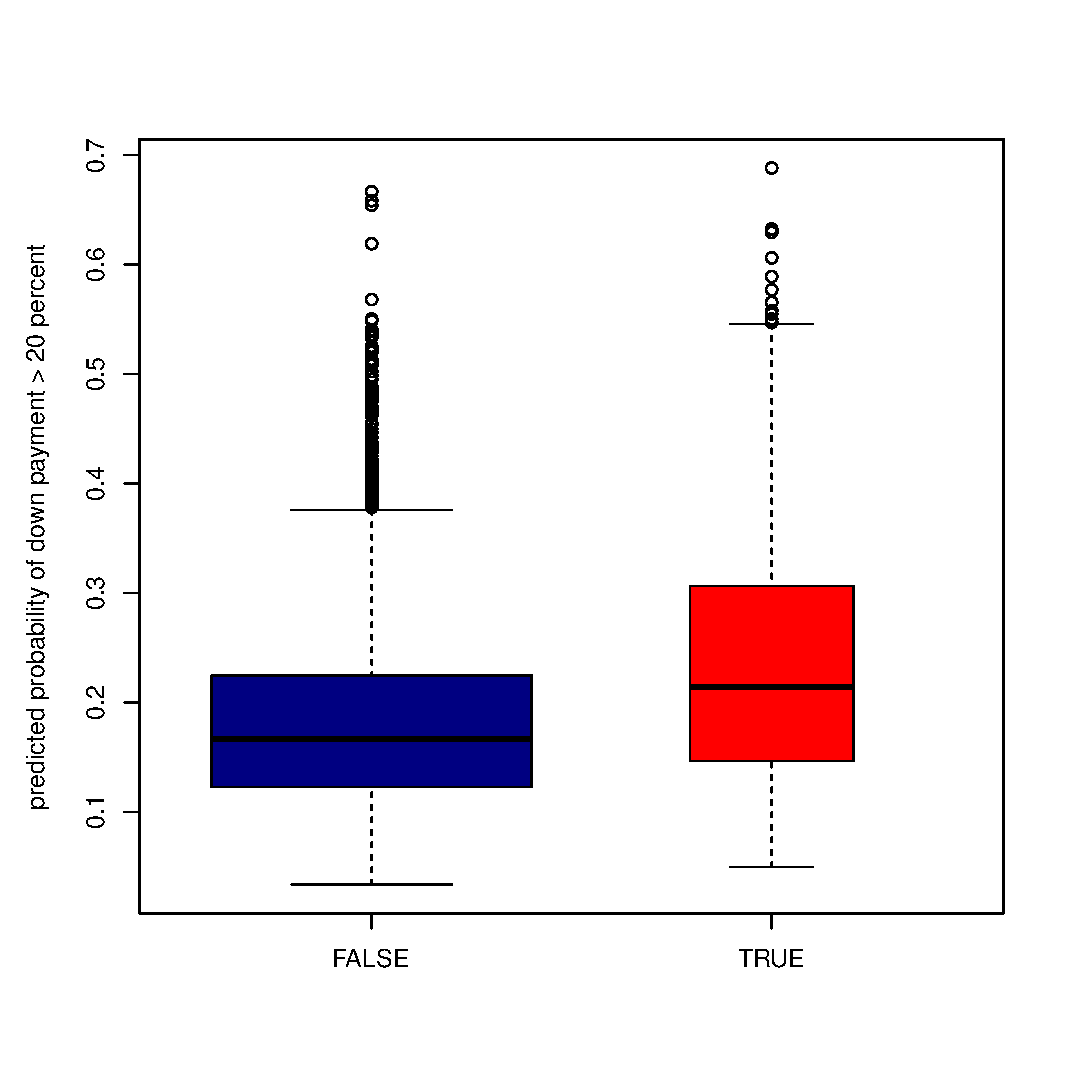
\includegraphics[scale=.5]{oos_lt100k.eps}
    \caption{Prediction Results for Homes $<100k$}
    \label{fig:oos_lt100k}
  \end{subfigure}
  \hfill
  \begin{subfigure}[b]{0.49\textwidth}
    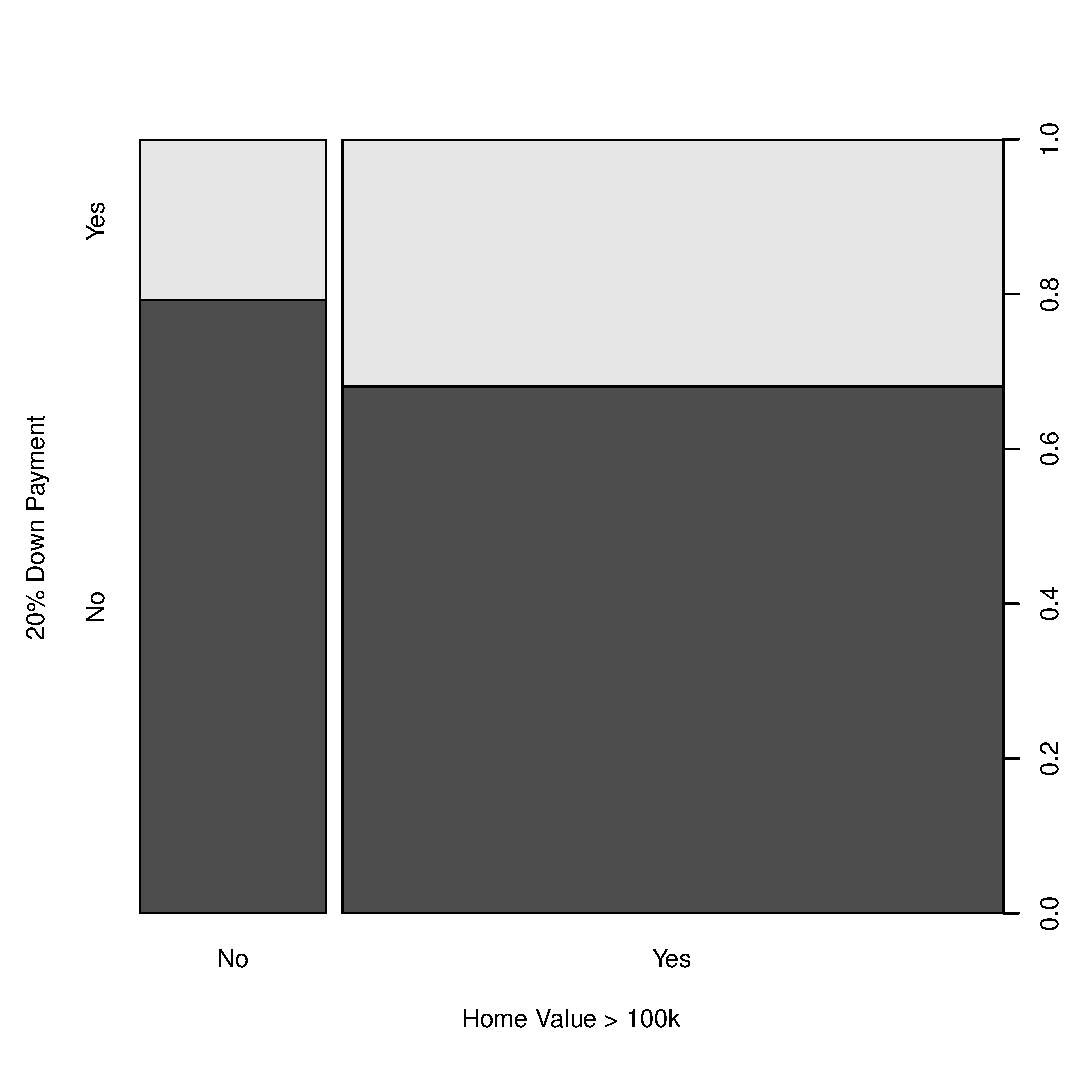
\includegraphics[scale=.5]{home_value_vs_20_down.eps}
    \caption{$20\%$ Down-Payment vs. Home Value}
    \label{fig:value_20dwn}
  \end{subfigure}
  \caption{Down-Payment Predictions}
\end{figure}

\subsection{Sample Predictions on Homes $>100k$}

One possibile explanation for the model's poor performace is that the training and out-of-sample data sets are fundamentally different. The class of purchasers for expensive homes could be different enough from the class of purchasers for inexpensive homes that calibrating the model on the former set does not tell us anything about the latter set. To see if this is the case, we train the model on a sub-sample of home buyers who only purchase homes $>$ 100k and predict for other home buyers who also purchase expensive homes.

Since a random sampling is performed on each iteration the $R^2$ for both the model and the out-of-sample prediction vary.  However, again we see that $R^2$ hovers around $\sim10\%$ with an out-of-sample $R^2$ anywhere between $\sim[1\%,18\%]$.  Figure~\vref{fig:oos_sample_gt100k} shows the result of one such run.  Again it seems to indicate that our prediction of down-payments $<20\%$ tends to be more accurate than our prediction of those $>20\%$.  However, both the mean and 1st/3rd quartiles for the prediction for a $>20\%$ down-payment are a bit higher, indicating that the model is slightly better, but, by no measure good, with these higher-priced homes.

This does indicate that perhaps the training sample we used in the prior section was too fundamentaly different from the prediction sample to make meaningful forecasts, and that training the model on a random sample of all homeowners would be a better strategy.

\begin{figure}[!htb]
  \centering
  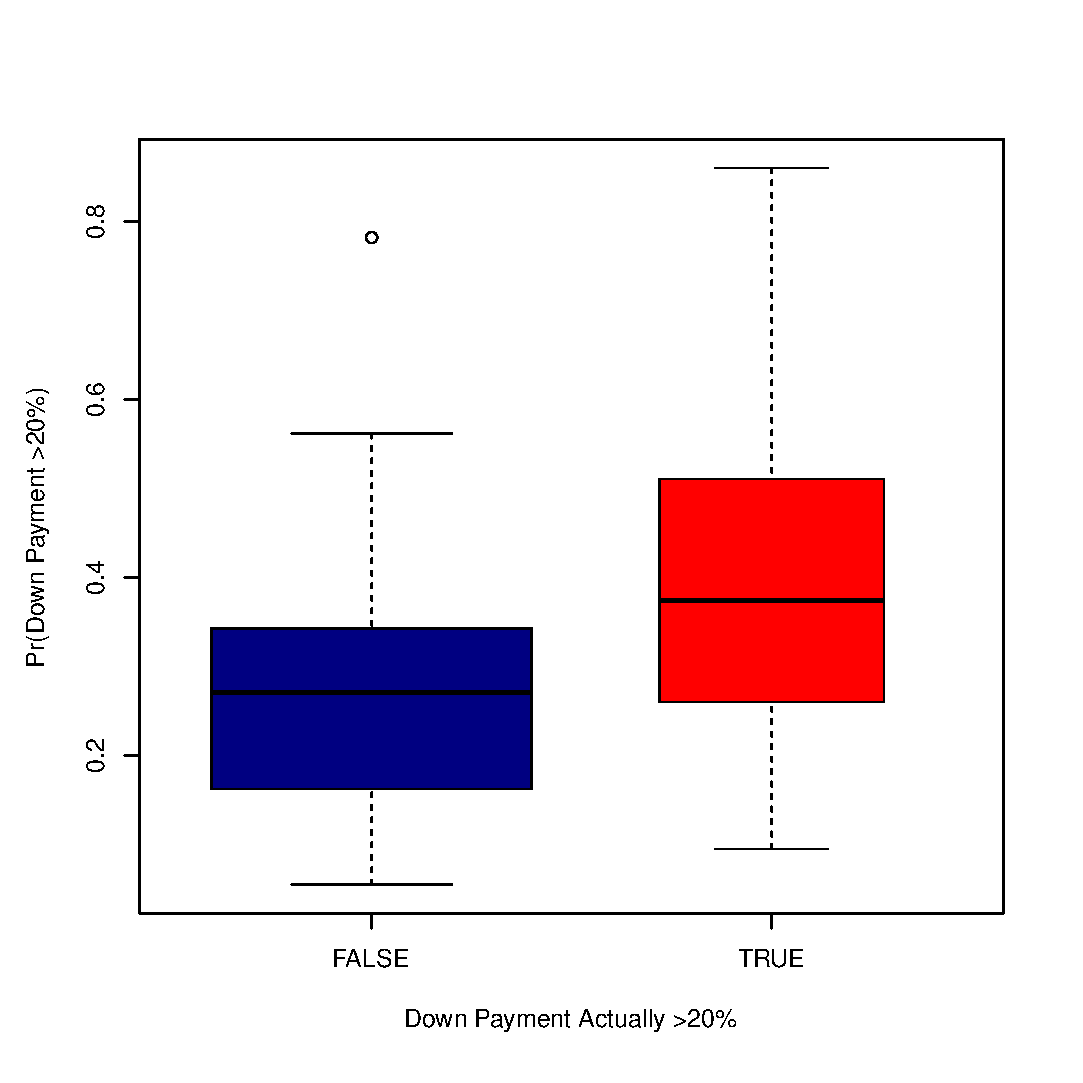
\includegraphics[scale=.5]{oos_subsample_100k.eps}
  \caption{Prediction Results for Out-of-Sample Homes $>100k$}
  \label{fig:oos_sample_gt100k}
\end{figure}

\end{document}
